\documentclass[12pt]{amsbook}
\usepackage[utf8]{inputenc}
\usepackage{amsmath}
\usepackage{amssymb}
\usepackage[english]{babel}
\usepackage{amsthm}
\usepackage{mathtools}
\usepackage{tikz-cd}
\usepackage[margin=1.4in]{geometry}
%\usepackage[nottoc]{tocbibind}
\usepackage{faktor}
\usepackage{cleveref}
\usepackage{helvet}
%\usepackage{titlesec}
%\usepackage{lipsum}

%\titleformat{\chapter}[display]
  %{\normalfont\bfseries}{}{0pt}{\Large}


% For shifting text a bit to compensate for binding
%\usepackage[a4paper,width=150mm,top=25mm,bottom=25mm,bindingoffset=6mm]{geometry}


\newcommand\phtpy{\stackrel{\mathclap{\normalfont\mbox{\small{p}}}}{\sim}}
\newcommand\htpy{\mathrel{\stackrel{\makebox[0pt]{\mbox{\normalfont\tiny p}}}{\sim}}}

\title{The naive homotopyclasses of k-scheme endomorphisms of \(\mathbb{P}^1\) admits a commutative monoid structure}
\author{Torgeir Aambø}
\date{January 2019}

\theoremstyle{definition}

\newtheorem*{theorem*}{Theorem}
\newtheorem*{lemma*}{Lemma}
\newtheorem*{corollary*}{Corollary}
\newtheorem*{definition*}{Definition}
\newtheorem*{remark*}{Remark}
\newtheorem{theorem}{Theorem}[section]
\newtheorem{lemma}{Lemma}[section]
\newtheorem{proposition}{Proposition}[section]
\newtheorem{example}{Example}[section]
\newtheorem{construction}{Construction}[section]
\newtheorem{corollary}{Corollary}[section]
\newtheorem{definition}{Definition}[section]
\newtheorem{remark}{Remark}[section]

\usepackage{nomencl}
\makenomenclature
\renewcommand{\nomname}{List of Symbols}
\setlength{\nomlabelwidth}{2.5cm}



\begin{document}


\newcommand{\HRule}{\rule{\linewidth}{1mm}}

\vspace*{\stretch{1}}
\noindent\HRule
\begin{center}
  \huge
  \noindent A naive homotopy theory for schemes\\ [7mm]
  %\noindent The naive homotopy classes of k-scheme endomorphisms of \(\mathbb{P}^1\) admits a commutative monoid structure \\ [7mm]
  \large
  \noindent\emph{Torgeir Aambø}
\end{center}
\noindent\HRule
\vspace*{\stretch{2}}
\begin{center}
\Large\textsc{Institutt for matematiske fag --- NTNU 2019}
\end{center}



\nomenclature[1]{$\longrightarrow$}{An arrow}
\nomenclature[2]{\(\htpy\)}{Pointed naive homotopy}
\nomenclature[3]{\(\cong\)}{Isomorphism (isomorphic)}
\nomenclature[4]{\(R^{\times}\)}{The set of units in \(R\)}
\nomenclature[5]{UFD}{Unique factorization domain}
\nomenclature[6]{\([a_{i,j}]_{i,j}\)}{Matrix with \(a_{i,j}\) at the \(i,j\)-th entry}
\nomenclature[7]{\(X \times Y\)}{The cartesian product of X and Y}

\nomenclature[8]{$A \coprod B$}{Disjoint union of $A$ and $B$}
\nomenclature[9]{\(\displaystyle \coprod_{i=0}^n A_n\)}{Disjoint union \(A_1 \coprod A_2 \coprod \dots  \coprod A_n\)} 

%\maketitle 

\frontmatter

\section*{Abstract}
In this thesis we attempt to understand naive homotopy theory and the naive homotopy classes of k-scheme endomorphisms of the projective line. We will use this to understand Christoph Cazanaves construction of the commutative monoid structure on these homotopy classes, and prove that this monoid is in fact commutative.  

\section*{Acknowledgements}
This thesis is the product of my bachelor studies in mathematics at the Norwegian University of Science and Technology (NTNU). I want to thank my supervisor Gereon Quick for helping me with the thesis, and for helping me with my studies in general at NTNU.


\tableofcontents

\section*{Introduction}
%
In topology, the notion of \emph{homotopy} characterizes the similarity of functions on topological spaces. A topological homotopy uses a topological space to say when two functions between topological spaces can be deformed into each other. 
It also characterizes when two spaces are similar enough to be continuously deformed into each other, called homotopy equivalence. A lot of the topological invariants often studied in topology are unchanged by homotopies, i.e. invariant under homotopy, making it a very strong and useful tool. 

Furthermore, using the equivalence classes generated by homotopy, this creates the notion of homotopy categories. The archetypal example is topological spaces together with homotopy classes of continuous maps. These are in fact such strong tools that mathematicians want to make an equivalent theory in other areas of mathematics. 

The classical method for doing so is to generalize the theory. This usually involves making the theory categorical and then applying it to other categories than the standard one we started with. This has been done with homotopy theory and the most used and recognized generalizations are called \emph{model categories} and \emph{\((\infty, 1)\)-categories}. The former is a purely categorical theory, while in the latter one needs higher category theory. 
We are not going to go deeper into these in this thesis, but we will be studying a special or simple case of the notion of homotopy in model categories. \\


We are going to explore a first approach to create a homotopy theory for schemes, called \emph{naive algebraic homotopy theory}. The general theory of the homotopy theory discussed in this thesis is called \emph{motivic homotopy theory} or \(\mathbb{A}^1\)-homotopy theory. 
The general theory is part of the generalization of homotopy theory to model categories, and one constructs the \(\mathbb{A}^1\)-homotopy category as the homotopy category of a model category for this theory. This construction is outside the scope of this thesis, but it can be useful to make a connection to this thesis if one later in life studies motivic homotopy theory and want intuition of something a little closer to home (which is of course normal topological homotopy theory). \\


The construction of our naive homotopy theory will be based heavily on the usual construction in topology, in the way that we change out the unit interval with something we can actually use in algebraic geometry. 
The unit interval is not an algebraic variety, so in the context of algebraic geometry we don't know how to use it. We are going to switch it out with the algebro-geometric version of the real line, or in general the simplest 1-dimensional scheme over a field, namely the \emph{affine line} \(\mathbb{A}^1\). This yields an interesting equivalence relation, however, it doesn't lead to the correct homotopy category for schemes. Nevertheless, Cazanave proves in \cite{Cazanave} that this naive version has some interesting properties when looking at the naive homotopy classes of endomorphisms of \(\mathbb{P}^1\). Cazanave proves that these classes admit a commutative monoid structure, and that the canonical morphism \([\mathbb{P}^1, \mathbb{P}^1]^N \to [\mathbb{P}^1, \mathbb{P}^1]^{\mathbb{A}^1} \) is a group completion. In this thesis we study the first result, that the homotopy classes form a commutative monoid, and we present a more detailed and slightly modified proof. 
\bigskip \\

The thesis is split into two chapters, each of them having their own sections. We give a short overview on the different parts of the thesis.

\textbf{Chapter 1} is titled naive homotopy and the scheme of rational functions, and this chapter consists mostly of definitions and comparisons. In this chapter we are defining and creating the building blocks for the rest of the thesis. We define what a naive homotopy is, what the scheme of rational functions is, what we mean by k-scheme morphisms, the projective line and more. 

\textbf{Chapter 2} is titled: Naive homotopy classes as a commutative monoid, and this chapter is where we prove the main theorem of the thesis. We start by constructing a monoid operation, and then show that the naive homotopy classes defined in chapter 1, together with this operation form a commutative monoid. 
\bigskip \\

For this thesis \(k\) is always a field with characteristic not equal to \(2\). Any ring mentioned is always a commutative unital ring. 
 




%\printnomenclature
%\include{Nomenclature} %DOES NOT WORK ATM
\mainmatter
\chapter{Naive homotopy and the scheme of rational functions}
%\addcontentsline{toc}{chapter}{Naive Homotopy}
%
Before we start of with the theorems and proofs, we go through the most important definitions and constructions of the objects which we will be using throughout the thesis. We try to define these definitions and constructions in the most ``helpful'' way, i.e. to best understand the material presented. This means that there are many equivalent definitions out there which may work better in other scenarios. These definitions are of course built on other more basic definitions in algebraic geometry, ring theory and commutative algebra. For readers wishing to understand this thesis but not having seen the definitions of objects like sheaves or schemes, we have added these in Appendix A. There is also an easy example to see how schemes ``looks'' in the appendix to help build intuition.
%
%
\section{Naive homotopy}
%
As roughly explained in the introduction, naive homotopy theory is kind of the natural way to try to make topological homotopy theory work for schemes. We substitute the unit interval since it is not a scheme. 
We substitute it with the closest algebro-geometric object we have, namely \(\mathbb{A}^1(k)\), the affine line over a field viewed as a scheme. We have added example \ref{Ex:Complex affine line} in Appendix A to show how to construct this scheme when the field \(k=\mathbb{C}\). 
Example \ref{Ex:Complex affine line} also shows how this scheme works as a substitute for the unit interval (or equivalently the real line) by visualizing it as an actual line. The naive homotopy is then defined analogously to the topological homotopy we are familiar with. This was of course not precise at all, so we give the following proper definition.
%
\begin{definition}\label{Def:Naive Homotopy}
%
A naive homotopy is a morphism \(h: X \times \mathbb{A}^1 \longrightarrow Y\), such that the restrictions \(\sigma (h) := h_{|X\times \{0\}}\) is the source of the homotopy, and \(\tau (h) := h_{|X\times \{1\}}\) is the target of the homotopy. If \(X\) and \(Y\) are pointed spaces, with \(x_0\) and \(y_0\) as the respective base points, then we call \(h\) a pointed naive homotopy if its restriction to \(x_0 \times \mathbb{A}^1 = y_0\).
%
\begin{example}
%
Every monic polynomial \(P\in k^{\times}\) of degree n is naively homotopic to its leading term, i.e.
\begin{equation*}
    P(x) \htpy x^n \,.
\end{equation*}
%
\end{example}
%
\end{definition}
%
The object we want to study in this thesis is the naive homotopy classes of k-scheme endomorphisms of the projective line. To do this we look at another scheme carrying the same information. We will also soon define what we mean with the homotopy classes. The scheme we will look at is defined as follows.
%
%
\section{Pointed rational functions}
%
%
\begin{definition}\label{Def:Scheme of rational functions}
Let \(1 \leq n \in \mathbb{N}\) and \(k\) be a field. The scheme of rational function of degree \(n\) with coefficients in \(k\), denoted \(\mathcal{F}_n\), is the open subscheme of the affine space
%
\begin{equation*}
    \mathbb{A}^{2n} = \text{Spec}(k[a_0,\dots,a_{n-1},b_0,\dots, b_{n-1}])
\end{equation*} complementary to the hypersurface given by the equation 
%
\begin{equation*}
    \text{res}_{n,n}(x^n+a_{n-1}x^{n-1}+\dots+a_0, b_{n-1}x^{n-1}+\dots+b_0) = 0.
\end{equation*}
%
Here \(\text{res}_{n,n}\) is the resultant function, i.e. the determinant of the Sylvester matrix given by the two polynomials \(x^n+a_{n-1}x^{n-1}+\dots+a_0 \) and \(b_{n-1}x^{n-1}+\dots+b_0\). We have given the definition of the Sylvester matrix in Appendix A \ref{Def:Sylvester matrix}. By convention, \(\mathcal{F}_0=\text{Spec}(k)\)
%
\end{definition}
%
\begin{definition}\label{Def:R-point}
%
Let \(R\) be a \(k\)-algebra, and \(0 \leq n \in \mathbb{N}\). An \(R\)-point of \(\mathcal{F}_n\) is a pair of polynomials \((A,B) \in R[x]\times R[x]\), with
%
\begin{enumerate}
    \item A is a monic polynomial of degree n
    \item B is of degree strictly less than n
    \item \(\text{res}_{n,n}(A,B) \in R^{\times}\), i.e it is invertible in R. 
\end{enumerate}
%
Such a point will be denoted by \(\frac{A}{B}\) and will be called a pointed rational function of degree \(n\) with coefficients in \(R\). The set of R-points in \(\mathcal{F}_n\) is denoted by \(\mathcal{F}_n(R)\).
%
\end{definition}
%
\begin{remark}\label{rm:invertability}
%
We force the resultant to be invertible because of the fact that two polynomials share a common root if and only if the resultant of the two polynomials is zero \cite[Corollary 1.8]{Janson}. Since a k-algebra is a vector space (remember that k is a field), non-zero determinant and invertability is equivalent. 
%
\end{remark}
%
These definitions are not very easy to understand, so we give a quick example of how to find R-points, or at least how to check if a pair of polynomials is an R-point. 
%
\begin{example}\label{Ex:R-point}
%
Let \(k=\mathbb{Z}/3\) and \(n=2\). Then \(\mathcal{F}_2\) is the subscheme of \(\text{Spec}((\mathbb{Z}/3)[a_0,a_1,b_0,b_1])\) complementary to the hypersurface spanned by the equation 
%
\begin{equation*}
%
    \text{res}_{2,2}(x^2+a_1x+a_0, b_1x+b_0) = \text{det}
%
    \begin{bmatrix}
    a_0 & b_0 & 0 \\
    a_1 & b_1 & b_0  \\
    1 & 0 & b_1
    \end{bmatrix}
%
= a_0 b_1^2 + a_0 b_0 b_1 - b_0^2.
%
\end{equation*}
%
Thus \(\mathcal{F}_2 = \text{Spec}(\mathbb{Z}/3[a_1,a_0,b_1,b_0])\setminus \langle a_0 b_1^2 + a_0 b_0 b_1 - b_0^2 \rangle \).
%
Now we can construct an \(\mathbb{Z}/3\)-point of \(\mathcal{F}_2\) by taking \((f,g)=(x^2+2x+2, x+2)\in \mathbb{Z}/3[x] \times \mathbb{Z}/3[x]\). Here f is monic and of degree 2, and g is of degree strictly less than 2, i.e. 1. Now all we need to check is that the resultant of the two polynomials is invertible in \(\mathbb{Z}/3\), which is shown by
%
\begin{equation*}
%
    \text{res}_{2,2}(f,g)= \text{det}
%
    \begin{bmatrix}
    2 & 2 & 0 \\
    2 & 1 & 2  \\
    1 & 0 & 1
    \end{bmatrix}
%
= 2.
%
\end{equation*}
%
which of course invertible in \(\mathbb{Z}/3\) since it is a field. \\
We conclude that \((f,g)= \frac{f}{g}\) is a \(\mathbb{Z}/3\)-point of \(\mathcal{F}_2\) i.e. a pointed rational function of degree 2 with coefficients in \(\mathbb{Z}/3\).
%
\end{example}
%
%
\section{Projective space}
%
The object we want to study in this thesis is \(\mathbb{P}^1\), or rather endomorphisms of \(\mathbb{P}^1\). The reader may know this object already, and even though the definition we are using is a bit more complicated, the same intuition still works. Later in the chapter we want to say that a k-scheme endomorphism of \(\mathbb{P}^1\) contains the same information as a pointed rational function. To do so we first need to define the projective line as a scheme, and to do that we need to define \(\text{Proj}(-)\). In \ref{Def:Spectrum of a ring} in appendix A, we define \(\text{Spec}(-)\). They are not extremely different, but to create projective structure one often need a little more work and restrictions. It may be helpful for the reader to use intuition about real n-space \(\mathbb{R}^n\) and the projective n-space \(\mathbb{RP}^n\) when thinking about Spec(R)  and Proj(S). Since \(\text{Proj}(S)\) is a scheme, it locally looks like an affine scheme isomorphic to \(\text{Spec}(R)\) for some R, which is is similar to how \(\mathbb{RP}^n\) looks like \(\mathbb{R}^n\) locally. 
%
\begin{definition}\label{Def:Homogeneous element}
%
A homogeneous element in a graded ring \(S= \bigoplus S_i\) is an element only contained in one of the \(S_i\)'s.
A homogeneous ideal of S is an ideal generated by a set of homogeneous elements. 
%
\end{definition}
%
\begin{construction}\label{Proj construction}
%
%
Let S be a graded ring, with \(S=\displaystyle \bigoplus_{i\geq 0} S_i\) as the direct sum decomposition. We define \(\text{Proj}(S)\) as just a set to be the set of homogeneous prime ideals not containing the irrelevant ideal \(S_+=\displaystyle \bigoplus_{i>0}S_i\). We then augment this set with the Zariski topology to form a topological space. We do this by defining the closed subsets to be 
%
\begin{equation*}
    V(A) = \{P\in \text{Proj}(S)|A\leq P\}
\end{equation*}
%
where \(A\) is a homogeneous ideal of S.

The final piece missing is to construct a structure sheaf. We do this by defining the local ring on every open set \(U\) to be the set of all functions 
%
\begin{equation*}
%
    f:U\longrightarrow \bigcup_{P\in U}S_{(P)}
%
\end{equation*}
%
where \(S_{(P)}\) is defined to be the subring of the ring of fractions of homogeneous elements of the same degree such that:
%
\begin{enumerate}
%
    \item \(f(P)\in S_{(P)}\)
    \item There exist an open subset \(V \subset U\) containing \(P\) and two homogeneous elements \(s,t\) of the same degree such that for each prime ideal Q of V
%
    \begin{enumerate}
        \item t is not in Q
        \item \(f(Q) = \frac{s}{t}\).
    \end{enumerate}
%
\end{enumerate}
%
\end{construction}
%
\begin{definition}\label{Def:Projective n-space}
%
Let \(R\) be a commutative ring with identity. We define the projective n-space over \(R\) to be the scheme
%
\begin{equation*}
    \mathbb{P}_R^n = Proj(R[x_0, \dots, x_n]).
\end{equation*}
%
Note that by our definition of \(\text{Proj(-)}\) we need a grading of the polynomial ring \(R[x_0,\dots,x_n]\). We define this by letting each \(x_i\) have degree \(1\) and each element \(r\in R\) to have degree \(0\). 
%
\end{definition}
%
Event though this definition is really complicated and seems fairly unmotivated, the definition formalizes \(\mathbb{P}^1\) being \(\mathbb{A}^1\) with a point at infinity. We can still use the usual intuition and notation, for example projective coordinates. Since we are looking at pointed rational functions, we define our base point to be \(\infty = [0:1] \in \mathbb{P}^1\).
%

\section{Morphisms of schemes}
%
By \cref{Def:Affine scheme} in Appendix A, an affine scheme consists of a set, with a topology and a sheaf of rings, i.e. a locally ringed topological space. Therefore to define a map of affine schemes, we would want it to respect these three structures. We should require it to be a map of sets, that is continuous and carrying some information about the sheaf. We also want morphisms of affine schemes \(\text{Spec}(S) \to \text{Spec}(R)\) to correspond exactly with ring morphisms \(R \to S\) since Spec(-) is a covariant functor. Since schemes are locally just affine schemes, we want general morphisms of schemes to locally act as morphisms of affine schemes. We define a morphism of schemes by the sequence of definitions given in  \cite[Def 6.2.1, 6.3.1, 6.3.3]{Vakil}. 

\begin{definition}
Let X and Y be ringed spaces. A morphism of ringed spaces \(\delta : X \to Y \) is a continuous map of the underlying topological spaces together with a map \(\mathcal{O}_{Y} \to \delta_*\mathcal{O}_{X}\) which we think of as a pullback map. 
\end{definition}

\begin{definition}
Let X and Y be locally ringed spaces. A morphism of locally ringed spaces \(\delta : X \to Y \) is a morphism of ringed spaces such that the induced map on the stalks \(\mathcal{O}_{Y, q} \to \mathcal{O}_{X, p}\) sends the maximal ideal to the maximal ideal. 
\end{definition}

\begin{definition}
Let X and Y be schemes. A morphism \(\delta : X \longrightarrow Y \) as locally ringed spaces is called a morphism of schemes. 
\end{definition}

This definition of a scheme morphism is not very useful for us. We are interested in morphisms between schemes over the same field \(k\), and not arbitrary schemes. 

\begin{proposition}
An S-scheme morphism \(f: X \to \mathbb{P}^1\), where \(X\) is an S-scheme, is equivalent to a choice of an invertible sheaf and two global sections \(s_0 = f^*(x_0), s_1 = f^*(x_1)\) generating the sheaf. Here \(x_0\) and \(x_1\) are homogeneous coordinates of \(\mathbb{P}^1\). 
%
\begin{proof}
A good proof of this can be found in \cite[Thm 7.1]{hartshorne} or \cite[Cor 13.33]{Wedhorn-Gortz}. 
\end{proof}
\end{proposition}
%
In \cite[Remark 13.34]{Wedhorn-Gortz} Wedhorn and Görtz give a quite explicit description of the map \(f: X(k) \to \mathbb{P}_k^1(k)\) when S (as in the previous proposition) is an affine scheme over a field, i.e. \(S = \text{Spec}(k)\). As above such a morphism correspond to an invertible sheaf \(\mathcal{L}\) and two global sections \(s_0\) and \(s_1\). They argue that there exists two unique elements \(\alpha_0 , \alpha_1 \in k\) such that \(s_0(x) = \alpha_0 s_1(x)\) and \(s_1(x) = \alpha_1 s_0(x)\). Then the map \(f\) is defined by mapping \(x \mapsto [\alpha_0 : \alpha_1]\) and denoting this point by \([s_0(x) : s_1(x)]\). \\
Now this starts to look more like a map we are familiar with from topology or from varieties. We don't want morphisms from any k-scheme X, so in the next section we describe the endomorphisms of \(\mathbb{P}^1\). 
%
\section{Endomorphisms of the projective line}
%
\begin{proposition}\label{Prop:Equivalent notions of morphisms}
%
A pointed k-scheme morphism  \(f: \mathbb{P}^1 \longrightarrow \mathbb{P}^1\) is equivalent to a non-negative integer \(n\) together with a pointed rational function \(\frac{A}{B}\in \mathcal{F}_n(k)\). The integer \(n\) is called the degree of \(f\), and is denoted \(\text{deg}(f)\), and the resultant \(\text{res}_{n,n}(A,B)\in k^{\times}\) is called the resultant of f, denoted \(\text{res}(f)\).
%
\begin{remark}\label{rm:connection between k-s morph and rat func}
%
This proposition tells us the connection between the usual notion of k-scheme morphisms between projective space and the previously defined \(k\)-points of \(\mathcal{F}_n\).
%
\end{remark}
%
%
\begin{proof}
%
A pointed endomorphism of the projective line is defined by a rational function \(f=\frac{f_1}{f_0}:\mathbb{P}^1\longrightarrow \mathbb{P}^1\), with \(f_1\) and \(f_0\) coprime polynomials and \(f_1\) of some degree \(n\) sending \(\infty \mapsto \infty\). This we know since \(f\) is a map that sends

%%%%%%%%%%%%%%%%%%%%%%%%%%%%%%%%%%%%%%%%%%%%%%%%%%%%
\iffalse
Since \(f(\infty)=\infty\), we may consider the restriction \(f_{|\mathbb{A}^1} = f_0 : \mathbb{A}^1 \to \mathbb{A}^1 \). This is given by a polynomial \(f_0 = A\) of some degree, say m. 
\fi
%%%%%%%%%%%%%%%%%%%%%%%%%%%%%%%%%%%%%%%%%%%%%%%%%%%%%

\([x_0:x_1] \mapsto [y_0:y_1]\) where at least one of the \(y_i\)'s are non zero, say \(y_0\). By continuity, there exist an affine neighbourhood \(U=\text{Spec(R)}\) for some ring R, such that 
%
\begin{equation*}
    f: U \to \mathbb{P}^1 - \{y_0 = 0\}
\end{equation*} \\
%
is a morphism where \(y_0, y_1\) are the homogeneous coordinates. We can identify \(\mathbb{P}^1 - \{y_0 = 0\}\) with \(\mathbb{A}^1\) via the maps \([a_0:a_1] \to [\frac{a_0}{a_0}:\frac{a_1}{a_0}] = [1:\frac{a_1}{a_0}] \to \frac{a_1}{a_0}\). \\
Now we have a map 
%
\begin{equation*}
    g_0 = f_{|U} : U \longrightarrow \mathbb{A}^1 \,, 
\end{equation*} \\
%
where \(g_0\) is a regular function, i.e. a global section of the structure sheaf on \(U\). This is given by a fraction of homogeneous elements of \(k[x]\), i.e. a fraction \(\frac{f_1}{f_0}\) of two polynomials with \(\text{deg}(f_0) \leq \text{deg}(f_1)\). Thus when we go back to the homogeneous coordinates we have \(f(x) = [f_0(x):f_1(x)]\) for all \(x\in U\). By continuity we can extend this such that it holds for all \(x \in \mathbb{P}^1\) as long as the two polynomials never vanish at the same time, i.e. they are coprime. By abuse of notation, we can write this function \(f = [f_0:f_1] = \frac{f_1}{f_0}\). \\
We now have a rational function of two polynomials, where they are coprime, i.e. have nonzero resultant and satisfy our degree requirement. The only thing missing is the monic condition, but since \(f_1\) has coefficients in our field \(k\), we can divide by the first coefficient to make it monic. We call the number \(n = \text{deg}(f_1)\) the degree of our rational function. and we say \(f_1 = A\) and \(f_0 = B\) to get the element \(\frac{A}{B}\in \mathcal{F}_n(k)\). 
%
\end{proof}
%
\end{proposition}
%
\begin{remark}
The same argument also works if we use \(k[t]\) instead of \(k\). Thus, in the same way as above, a naive homotopy is equivalent to an element \(h(t) \in \mathcal{F}_n(k[t])\). \footnote{In other words, a naive homotopy is  a \(k[t]\)-point in \(\mathcal{F}_n\).}   
\end{remark}
%%%%%%%%%%%%%%%%%%%%%%%%%%%%%%%%%%%%%%%%%%%
%\iffalse
%\begin{proof}
%
%Each morphism of schemes:
%\begin{center}
%    \begin{tikzcd}
%Spec(R) \arrow[rr, "f"] &  & {Spec(k[a_0,\dots a_{n-1},b_0,\dots,b_{n-1}])\setminus H}
%    \end{tikzcd}
%\end{center}
%Gives us a morphism \(\Bar{f}:k[a_0,\dots a_{n-1},b_0,\dots,b_{n-1}])\setminus H\longrightarrow R\). This morphism sends a polynomial in the \(2n\) variables to the evaluation of the polynomial in \((r_0,\dots,r_{n-1},s_0,\dots,s_{n-1})\in R^{2n}\).
%
%\end{proof}
%\fi
%%%%%%%%%%%%%%%%%%%%%%%%%%%%%%%%%%%%%%%%%%%
%
\begin{definition}\label{Def:Pointed naive homotopyclass}
%
We say that two pointed rational functions \(f\) and \(g\) lie in the same pointed naive homotopy class if there exist a finite sequence of naive homotopies, \(\{h_i\}\) with \( 0 \leq i \leq N \), such that
%
\begin{equation}
\sigma(h_0) = f, \quad \tau(h_N) = g,
\end{equation} 
%
and, they are connected, i.e.
%
\begin{equation}
\tau(h_i) = \sigma(h_{i+1}), \quad \forall i \in [0,N-1] .
\end{equation}
%
We denote two pointed rational functions being in the same pointed naive homotopy class by \(f \htpy g\), and the set of pointed naive homotopy classes by \([\mathbb{P}^1, \mathbb{P}^1]^N\). Hence we have
%
\begin{equation}
\coprod_{0\leq n} \faktor{\mathcal{F}_n(k)}{\htpy}   = [\mathbb{P}^1, \mathbb{P}^1]^N.
\end{equation}
%
\end{definition}
%
\begin{corollary}\label{Cor:when does two functions lie in the same homotopyclass}
Two pointed rational functions are in the same naive homotopy class if and only if they have the same degree.
%
\begin{proof}
This follows directly from \cref{Prop:Equivalent notions of morphisms}.
\end{proof}
%
\end{corollary}
%
%%%%%%%%%%%%%%%%%%%%%%%%%%%%%%%%%%%%%%%%%%%%
\iffalse
\begin{proof}
[SKETCH] A polynomial\(A=\frac{x^n+a_{n-1}x^{n-1}+\dots+a_0}{b_0}\) is homotopic to its leading term, i.e. \(\frac{x^n}{b_0}\).
Let \(B= b_{n-1}x^{n-1}+\dots+b_0\), then \(A \htpy \frac{x^n}{b_0} \htpy \frac{x^n}{B}\).\\
blabla proof
\end{proof}
\fi
%%%%%%%%%%%%%%%%%%%%%%%%%%%%%%%%%%%%%%%%%%%%
%
\begin{corollary}\label{cor:htpyclasses split degreewise}
The set of pointed naive homotopy classes \([P^1, P^1]^N\) splits into a disjoint union of its degreewise components, i.e. 
\begin{equation*}
    [\mathbb{P}^1,\mathbb{P}^1]^N = \coprod_{n\geq 0}[\mathbb{P}^1,\mathbb{P}^1]_n^N.
\end{equation*}
\begin{proof}
Follows directly from \cref{Cor:when does two functions lie in the same homotopyclass}.
\end{proof}
\end{corollary}
%
\begin{remark}\label{rm:reformulation to connected components}
Later in the thesis we will see that it is more convenient to use the naive connected components of our scheme of pointed rational functions. Hence we need to define what we mean by naive connected components. We construct them generally by taking a functor from the category of k-algebras to the category of sets  
\begin{equation*}
    \mathcal{G}:Alg_k \longrightarrow \mathcal{S}et .
\end{equation*}
\end{remark}
%
And we define a new functor
%
\begin{equation*}
    \pi_0^N\mathcal{G}:Alg_k \longrightarrow \mathcal{S}et
\end{equation*}
%
which takes a k-algebra R and gives it the coequalizer of the double arrow 
%
\begin{equation*}
    \mathcal{G}(R[t])\rightrightarrows \mathcal{G}(R)
\end{equation*}
%
given by evaluating at \(t=0\) and \(t=1\). We define \(e_a\) the map that evaluates a function at a point a, and thus we give it the coequalizer of \(e_0, e_1\). 
%
Remember that the coequalizer in the category of sets is the smallest equivalence relation such that the two functions are pointwise equal in the equivalence classes generated by said relation.  \\
This can be thought of as sending a k-algebra to the polynomial connected components on that algebra. 
%
%Thereby in our situation, it means they lie in the same naive homotopy class.
A scheme can be thought of as a functor from k-algebras to sets. In fact by \cite[Prop. VI-2]{Eisenbud-Harris}, the category of k-schemes is equivalent to a full subcategory of the functor category between k-algebras and sets. If we let the \(\mathcal{G}\) be the scheme \(F_n\) interpreted as a functor, then we get the new functor

\begin{equation*}
    \pi_0^N\mathcal{F}_n : Alg_k \longrightarrow \mathcal{S}et .
\end{equation*}
This sends the field \(k\) to the coequalizer of  
\begin{equation*}
    \mathcal{F}_n(k[t])\rightrightarrows \mathcal{F}_n(k), 
\end{equation*}

i.e. the object 

\begin{equation*}
    \faktor{\mathcal{F}_n(k)}{\{ e_0(h(t)) \sim e_1(h(t)) \, | \, \forall h(t) \in \mathcal{F}_n(k[t])\}}. 
\end{equation*}

Recall that we showed that elements in \(\mathcal{F}_n(k[t])\) are naive homotopies, and hence the coequalizer becomes 

\begin{equation*}
     \faktor{\mathcal{F}_n(k)}{\{ \sigma(h) \sim \tau(h) \, | \, \forall h : \mathbb{P}^1 \times \mathbb{A}^1 \to \mathbb{P}^1\}}, 
\end{equation*}
which are exactly the naive homotopy classes. 
Since we have shown that the homotopy classes of pointed rational functions split degreewise, the same proposition gives us a bijection
\begin{corollary}\label{cor:connected components is homotopy classes}
\begin{equation*}
    [\mathbb{P}^1, \mathbb{P}^1]_n^N \cong (\pi_0^N\mathcal{F}_n)(k).
\end{equation*}
\end{corollary}

%
Intuitively this should not be that difficult to convince ourselves of. We send our field \(k\) as an algebra over itself to the  homotopy class of degree \(n\) pointed rational functions on \(k\) by our constructed functor. Since \(\mathcal{F}_n(k[t])\) consists of naive homotopies, we get our naive connected components by evaluating every naive homotopy on \(0\) and \(1\). These naive connected components are just the naive homotopy classes. By proposition \ref{Prop:Equivalent notions of morphisms} we already have that every k-scheme endomorphism of the projective line is a degree n rational function, and since they are isomorphic as sets, they will also have the same connected components i.e. naive homotopy classes. To summarize, all this does is to reformulate what it means to be a naive homotopy class. It just means that two functions live in the same homotopy class if they can be connected by a path. \footnote{This also means that paths is this space is the same as homotopies.} 

%
\chapter{Naive homotopy classes as a commutative monoid}
%
To prove that the naive homotopy classes of the pointed rational functions in fact admits a commutative monoid, we need to give it a monoid operation. We are going to do so by first constructing a monoid structure on the disjoint union scheme \(\mathcal{F}=\displaystyle \coprod_n \mathcal{F}_n\). This will induce a monoid structure on its naive connected components \((\pi_0^N\mathcal{F}_n)(k)\), which we have seen is isomorphic to \([\mathbb{P}^1,\mathbb{P}^1]^N_n\) in the end of the previous chapter. 

%
%

\section{The monoid operation}
%
Two polynomials \(A\) and \(B\), of respective degrees \(n\) and \(m\) with no common zeroes uniquely define two polynomials \(U\) and \(V\), with respective degrees \(k\), \( l\) such that \(k < m\) and \(l < n\). These polynomials satisfy a unique Bézout-relation \(AU+BV=1\). This should feel familiar if the reader has seen some elementary number theory. The proof often uses the extended Euclidean algorithm backwards, as done in \cite[Thm 3.6.1]{hsu}. We are going to use this to construct a graded monoid structure on \(\mathcal{F}\). 
%
\begin{definition}\label{def:monoid operation}
For a pointed rational function \(\frac{A}{B}\in \mathcal{F}_n(k)\) let  \(U, V \in k[x]\) be the uniquely defined polynomials such that \(AU+BV=1\). Let  \(\frac{A_1}{B_1}\in \mathcal{F}_n(k)\) and \(\frac{A_2}{B_2}\in \mathcal{F}_m(k)\) be two rational functions of respective degree \(n\) and \(m\), with Bézout relations \(A_1 U_1 + B_1 V_1 = 1\) and \(A_2 U_2 + B_2 V_2 = 1\). We define the addition \(\frac{A_1}{B_1}\oplus^N \frac{A_2}{B_2}\) to be the new function \(\frac{A_3}{B_3}\), where \(A_3\) and \(B_3\) is defined by:
\begin{equation*}
%
\begin{bmatrix}
    A_3 & -V_3 \\
    B_3 & U_3 
\end{bmatrix} = 
%
\begin{bmatrix}
    A_1 & -V_1 \\
    B_1 & U_1 
\end{bmatrix}\cdot
%
\begin{bmatrix}
    A_2 & -V_2 \\
    B_2 & U_2 
\end{bmatrix}.
%
\end{equation*}
%
We write \(\frac{A_1}{B_1}\oplus^N\frac{A_2}{B_2} = \frac{A_3}{B_3}\) . \\
%
\end{definition}
%
\begin{remark}\label{Rm:N-sums work as expected}
By their respective Bézout relations, both the matrices on the right hand side have determinant \(1\) and hence the newly produced matrix also has determinant \(1\). \(A_3\) is monic with degree \(n+m\), since both \(A_1\) and \(A_2\) monic and the degree of \(-V_1 B_2\) is less than \(n+m = deg(A_1 A_2)\). Also just for degree reasons of the polynomials used in the definition, \(deg(B_3)\langle deg(A_3)\). Thus the new polynomials \(A_3\) and \(B_3\) do in fact form a pointed rational function \(\frac{A_3}{B_3}\) of degree \(n+m\). \\
%
Since matrix multiplication is associative, this new monoid law \(\oplus^N\) is also associative. %
Note that even though we use additive notation, this operation on \(\mathcal{F}\) is not commutative. \footnote{ This is because matrix multiplication is non-commutative.} 
\end{remark}
 
%
\begin{remark}\label{rm:induces monoid on conn components}
%
As said in the beginning of the chapter, this induces a monoid structure on its naive connected components, namely \((\pi_0^N\mathcal{F}_n)(k)\) and thus also on \([\mathbb{P}^1,\mathbb{P}^1]^N\) since they are isomorphic. We denote the induced monoid operation on \([\mathbb{P}^1,\mathbb{P}^1]^N\) by the same symbol, \(\oplus^N\). 
%
\end{remark}
%
Lets give a short example on how this monoid operation works.
\begin{example}\label{Ex:Computing easy N-sums}
Let's calculate the sum \(\frac{x}{u}\oplus^N\frac{A}{B}\), where \(a\in k^{\times}\) and \(\frac{A}{B}\in \mathcal{F}_n(k)\). \\

First lets look at the Bézout relations on the rational functions. We have \(xU_1 + u V_1 = 1\), where \(\text{deg}(V_1) < \text{deg}(x) = 1 \, \implies V_1 = c, \, c \in k^{\times}\). This means that the product \(xU_1\) is constant, but \(x\) is non-constant and \(\text{deg}(U_1) < n\). Thus \(U_1 = 0\) and \(c = \frac{1}{u}\). Hence we get
%
\begin{align*}
\frac{x}{a}\oplus^N\frac{A}{B} 
&= \frac{xA - VB}{uA -UB} \\ 
&= \frac{xA - cB}{uA} \\
&= \frac{xA-\frac{B}{u}}{uA}. 
\end{align*}
%
\end{example}
%
%
\section{The Bézout matrix}
%
Bézout gave in the 18th century a way to form a nondegenerate symmetric matrix from two polynomials, or in our case from a pointed rational function. Translated over to algebraic geometry, he defined for every positive integer \(n\), a morphism between the scheme of degree \(n\) pointed rational functions, \(\mathcal{F}_n\), and the scheme of nondegenerate symmetric \(n\times n\)-matrices, \(\mathcal{S}_n\). 
%
\begin{definition}\label{def:Bezout matrix}
%
The Bézout matrix \(\text{Béz}_n(A,B)\) is the matrix given by the coefficients \(c_{p,q}\) in 
%
\begin{equation*}
%
    \delta_{A,B}(x,y) = \frac{A(x)B(y)-A(y)B(x)}{x-y} = \displaystyle \sum_{p,q=1}^n c_{p,q}x^{p-1}y^{q-1}.
%
\end{equation*}
%
Note that \(c_{p,q}=c_{q,p}, \forall p,q \in {1,\dots,n}\), hence \(\text{Béz}_n(A,B)\) is a symmetric matrix. 
%It is also nondegenerate because of Bézouts formula:
%
It is also invertible because of Bézouts formula:
\begin{equation*}
%
    \text{det}(\text{Béz}_n(A,B))=(-1)^{\frac{n(n-1)}{2}}\text{res}(A,B).
\end{equation*}
%
\end{definition}
%

%%%%%%%%%%%%%%%%%%%%%%%%%%%%%%%%%%%%%%%%%%%%%%%%%%%%%%%%%%%
%\iffalse
%\begin{definition}\label{def:Bezout form}
%We define the Bézout form of a degree \(n\) rational function \(f=\frac{A}{B}\) to be the symmetric bilinear form over \(R^n\) who's Gram matrix is the Bézout matrix \(B_n(A,B)\). We denote this form by \(\text{Béz}_n(f)\).
%\end{definition}
%\fi
%%%%%%%%%%%%%%%%%%%%%%%%%%%%%%%%%%%%%%%%%%%%%%%%%%%%%%%%%%%

\begin{definition}
We define the Bézout function to be the map that sends a pointed rational function to its Bézout matrix, i.e. 

\begin{center}
%
\begin{tikzcd}
\mathcal{F}_n(k) \arrow[rr, rightarrow, "B\Acute{e}z_n"] &  & \mathcal{S}_n(k) 
\end{tikzcd}

\begin{tikzcd}
\quad \quad \frac{A}{B} \, \arrow[rr, rightarrow, maps to] & & 
\text{Béz}_n(A,B).
\end{tikzcd}
%
\end{center}
\end{definition}
%

%
The last section will be devoted to showing that the Bézout function exactly distinguishes the naive homotopy classes we want.
%
%
\section{The main theorem}
%
The main result in this paper will be proving that the set of naive homotopy classes of k-scheme endomorphisms of the projective line is in fact a commutative monoid with the operation \(\oplus^N\) that we defined previously, i.e.
%
\begin{theorem}\label{thm:Main-theorem}
\(([\mathbb{P}^1, \mathbb{P}^1]^N,\oplus^N)\) is commutative. 
\end{theorem}
%
We split the proof of the main theorem into smaller lemmas. In short terms, we will prove that the Bézout function is an isomorphism on the naive connected components, and then prove that the scheme of non-degenerate symmetric matrices \(\mathcal{S}_n\) is a commutative monoid with direct sum as the operation. Direct sum of matrices N and M works by letting \(N\oplus M\) be the block diagonal matrix with N in the first block and M in the second. We will also use the naive connected components of \(\mathcal{S}_n\), i.e. \((\pi_0^N\mathcal{S}_n)(k)\), and these are constructed in exactly the same way as \((\pi_0^N\mathcal{F}_n)(k)\). We show in the last lemma that \(\mathcal{S}_n\) is commutative up to naive homotopy.\\
But first we define some notation we will be using. Let n be a positive integer and \(a_i \in K^{\times}\), we define
%
%%%%%%%%%%%%%%%%%%%%%%%%%%%%%%%%%%%%%%%%%%%%%%%%%%%%%%%%%%%
%\iffalse
% Cazanaves def
%\begin{equation*}\label{def:\langle a...a\rangle sym diag form}
%
%\langle a_1, \dots, a_n\rangle  \text{to be the diagonal symmetric bilinear form }  \langle a_i\rangle \oplus \dots \oplus \langle a_n \rangle 
%
%\end{equation*}
%
%\fi
%%%%%%%%%%%%%%%%%%%%%%%%%%%%%%%%%%%%%%%%%%%%%%%%%%%%%%%%%%%
%
% My Def

\begin{equation*}\label{def:diagonal matrix <a..a> }
%
\langle a_1, \dots, a_n \rangle  \text{ to be the diagonal matrix } \langle a_ i\rangle \oplus \dots \oplus \langle   a_n \rangle  ,
%
\end{equation*}
%
which is the matrix with \(a_i\) on the \(i,i\)-th place, and zero everywhere else. We also define 
%

\begin{equation*}\label{def:pointed rational function [a...a]}
[a_1,\dots,a_n] \text{ to be the pointed rational function } \frac{x}{a_1}\oplus^N \dots \oplus^N \frac{x}{a_n}.
\end{equation*}
%
\begin{lemma}\label{Lm:homotopy-lemma in S}
%
Let \(n\) be a positive integer. Then for any nondegenerate symmetric matrix \(S \in \mathcal{S}_n(k)\) there exists units \(a_1, \dots ,a_n\) s.t. \(S\) is homotopic to the diagonal matrix \(\langle a_1, \dots, a_n\rangle \).
%
\begin{proof} 
Any matrix \(S \in \mathcal{S}_n(k)\) is congruent to a diagonal matrix \(A\) by a matrix \(P\in SL_n(k)\). We can decompose \(P\) into elementary matrices and this forms our homotopy from \(S\) to a diagonal matrix. Then we get the units \(a_i = A_{i,i}\). \\
%
\end{proof}
%
\end{lemma}
%
\begin{lemma}\label{Lm:homotopy-lemma in F}
Let \(n\) be a positive integer. Then for any pointed rational function \(f\in \mathcal{F}_n(k)\) there exists units \(a_1, \dots, a_n\) s.t. \(f\) is homotopic to the pointed rational function \([a_1, \dots,a_n]\).
%
\begin{proof}
%This point is proven by induction on the degree of the function. \\
A rational function \(f \in \mathcal{F}_n(k)\) is tautologically equivalent to the \(\oplus^N\)-sum of some polynomials \(\frac{A_1}{u_1}, \dots , \frac{A_n}{u_n}\), where \(u_i \in k^{\times}\).\footnote{This is because of a natural continued fraction expansion that comes from the \(\oplus^N\) operation. See this expansion in \cite[Ex 3.3]{Cazanave}. The tautological sum decomposition is then the sum of the polynomials in the continued fraction expansion.} Therefore it is enough to prove the case where \(f\) is a polynomial. Every polynomial is naively homotopic to its leading term \cite[Ex 2.4]{Cazanave}, thus we can treat \(f\) as a monomial \(\frac{x^n}{u}\) where \(u\in k^{\times}\). The element \(\frac{x^n}{tx^{n-1}+u} \in \mathcal{F}_n(k[t])\) defines a naive homotopy between \(\frac{x^n}{u}\) and \(\frac{x^n}{x^{n-1}+u}\). The function \(\frac{x^n}{x^{n-1}+u}\) decomposes as the \(\oplus^N\)-sum \(x\oplus^N g\) for some \(g\in \mathcal{F}_{n-1}(k)\). From here we can repeat the process with the function \(g\), and after \(n\) steps get the decomposition we wanted.
%
\end{proof}
%
\end{lemma}
%
We now want to show that the Bézout function is an isomorphism. Three things need to be shown; injectivity, surjectivity and compatibility with the monoid structure.  
%

% 
%%%%%%%%%%%%%%%%%%%%%%%%%%%%%%%%%%%%%%%%%%%%%%%%%%%%%%%%%%%
% Cazanave's lemma
%\iffalse
%
%\begin{lemma}\label{lm:conjugate to block matrix}
%Let \(\frac{A}{B}\in \mathcal{F}_n(k)\) and let \(u\in k^{\times}\). \\
%The Bézout form of \(\frac{x}{u}\oplus^{N}\frac{A}{B}\) is conjugate to the block diagonal form \(\frac{x}{u}\oplus^{N}\text{Béz}_n(A,B)\) by an element \(P\in SL_{n+1}(k)\).
%\end{lemma}
%
%\fi
%%%%%%%%%%%%%%%%%%%%%%%%%%%%%%%%%%%%%%%%%%%%%%%%%%%%%%%%%%%

% My lemma
\begin{lemma}\label{lm:Bez respects monoid structure}
The Bézout function respects the monoid structure on naive connected components. 

\begin{proof}

To show this we use the fact from lemma  \ref{Lm:homotopy-lemma in F} that any degree \(n\) rational function \(f \htpy \frac{x}{u_1}\oplus^N \dots \oplus^N \frac{x}{u_n}\) for \(u_1,\dots , u_n \in k^{\times}\).  
%
If we can prove that we can split off one such simple function, then we are done. Let \(u = u_1\) and \(\frac{A}{B}= \frac{x}{u_2}\oplus^N \dots \oplus^N \frac{x}{u_n}\). Then \(f \htpy \frac{x}{u} \oplus^{N} \frac{A}{B}\).

By \cref{Ex:Computing easy N-sums} we know that \(\frac{x}{u}\oplus^{N}\frac{A}{B} = \frac{xA-\frac{B}{u}}{uA}\). From the construction of the Bézout form we then have:
%
\begin{align*}
     \delta_{xA-\frac{B}{u}, uA}(x,y) 
     &= \frac{(xA-\frac{B}{u})(x)(uA)(y)-(xA-\frac{B}{u})(Y)(uA)(x)}{x-y} \\
     &= \frac{((xA)(x)-\frac{B}{u}(x))(uA)(y)-((xA)(y)-\frac{B}{u}(x))(uA)(y)}{x-y} \\
     &= \frac{xA(x)uA(y)-B(x)A(y)-yA(y)uA(x)+B(y)A(x)}{x-y} \\
     &= \frac{xA(x)uA(y)-yA(y)uA(x)}{x-y}+\frac{B(y)A(x)-B(x)A(y)}{x-y} \\
     &= \frac{u(x-y)A(x)A(y)}{x-y}+\frac{A(x)B(y)-A(y)B(x)}{x-y} \\
     &= uA(x)A(y)+\delta_{A,B}(x,y).
\end{align*}
%
We can now look at the coefficients that define the Bézout matrix. Since we also know that A is a polynomial, we can write an explicit expression of \(A(x)A(y)\). We then have
%
\begin{align*}
  \sum_{0\leq p,q \leq n+1}b_{p,q}x^{p-1}y^{q-1}  
    &= \delta_{xA-\frac{B}{u}, uA}(x,y) \\
    &= uA(x)A(y)+\delta_{A,B}(x,y)\\
    &= uA(x)A(y) + \sum_{0\leq p,q \leq n}c_{p,q}x^{p-1}y^{q-1} \\
    &= u\sum_{0\leq p,q \leq n+1}a_{p,q}x^{p-1}y^{q-1} + \sum_{0\leq p,q \leq n}c_{p,q}x^{p-1}y^{q-1} \\
    &= \sum_{0\leq p,q \leq n+1}(ua_{p,q}+c_{p,q})x^{p-1}y^{q-1}\,,
\end{align*}
%
where we have set \(c_{n+1,n+1}=0\). \\
Since \(a_{n+1,n+1}=1\) (because A is monic \footnote{ We proved this in \cref{Rm:N-sums work as expected}.}), this shows that the \((n+1,n+1)\)-entry in the Bézout matrix of the sum is equal to \(u\), i.e. \(b_{n+1,n+1}=ua_{n+1,n+1}-c_{n+1,n+1} = u\). Since \(u\) is a unit, we can use it to get rid of all other entries in the corresponding row and column, just like in linear algebra. This leaves us with a matrix of the form:
%
\begin{equation*}
%
\begin{bmatrix}
    * & \dots & 0 \\
    \vdots & \vdots & \vdots \\
    0 & \dots & u
\end{bmatrix} .
%
%%%%%%%%%%%%%%%%%%%%%%%%%%%%%%%%%%%%%%%%%%%%%%%%%%%%%%%%%%%
% a_n matrix
%\iffalse
%\begin{bmatrix}
%    * & \dots & a_{n,1} \\
%    \vdots & \vdots & \vdots \\
%    a_{1,n} & \dots & u
%\end{bmatrix} 
%\fi
%%%%%%%%%%%%%%%%%%%%%%%%%%%%%%%%%%%%%%%%%%%%%%%%%%%%%%%%%%%
%
\end{equation*}
%
These row and column operations corresponds to paths (homotopies) in \(\mathcal{S}_{n+1}(k)\). We can then split off \(\langle u \rangle \) from the matrix to get the direct sum
%
\begin{equation*}
    \begin{bmatrix}
        * & \dots & 0 \\
        \vdots & \vdots & \vdots \\
        0 & \dots & u
    \end{bmatrix} 
=
    \begin{bmatrix}
    * & \dots & * \\
    \vdots & \vdots & \vdots \\
    * & \dots & *
\end{bmatrix} 
%
\oplus \langle u \rangle .
%
\end{equation*}
We can change the remaining \(n\times n\) matrix \([c_{i,j}+a_{i,j}(u-a_{n+1,j})]_{i,j}\) with a homotopy to get the matrix \([c_{i,j}]_{i,j}\). Finally we have 
%
\begin{equation}
%
    \text{Béz}(\frac{x}{u}\oplus^{N}\frac{A}{B}) \sim 
    \, \langle u \rangle \oplus \text{Béz}(\frac{A}{B}) =
    \text{Béz}(\frac{x}{u})\oplus \text{Béz}(\frac{A}{B}).
%
\end{equation}
%
Note that we have flipped the sum here without showing that it commutes. We do this to more easily see that it respects the monoid structure. The proof of commutativity is done on the next page. \\
This proves that we can factor out these simple functions from the homotopy decomposition of any function. The fact that \(\langle u \rangle =\text{Béz}(\frac{x}{u})\) will be shown in the next lemma. Thus we get:
\begin{equation}\label{Eq:Bezout decomposition}
%
    \text{Béz}(f)=\text{Béz}(\frac{x}{u_1}\oplus^N \dots \oplus^n \frac{x}{u_n}) \sim \text{Béz}(\frac{x}{u_1})\oplus \dots \oplus \text{Béz}(\frac{x}{u_n}) .
%
\end{equation}
%
We wanted to show that the Béz functions respects the monoid structure for any two rational functions \(f=\frac{A}{B}, g = \frac{C}{D}\). This follows easily from what we have already done. 

\begin{align*}
     \text{Béz}(f\oplus^N g)
     &= \text{Béz}(\frac{x}{u_1}\oplus^N \dots \oplus^n  \frac{x}{u_n}\oplus^N g) \\
     &\sim \text{Béz}(\frac{x}{u_1})\oplus \dots \oplus  \text{Béz}(\frac{x}{u_n})\oplus \text{Béz}(g) \\
     &\sim \text{Béz}(f)\oplus \text{Béz}(g).
\end{align*}
%
Everything in the proof is as noted done up to homotopy. This is the same as doing the proof up to path connected components, which is exactly what we wanted to show. 
\end{proof}
%
\end{lemma}
%
\begin{lemma}\label{lm:Bez surjection on naive path components}
The Bézout function is surjective on naive path components. 
%
\begin{proof}
As seen in \cref{Eq:Bezout decomposition} we can decompose the Bézout matrix of any rational function into simple bits. We now prove that the Bézout \(1 \times 1\) -matrix \(\text{Béz}(\frac{x}{u}) = \langle u \rangle \).
%
\begin{equation*}
   \langle u\rangle _{1,1} = \delta_{x,u}(x,y) 
   = \frac{x(x)u(y)-x(y)u(x)}{x-y} 
   = \frac{xu-yu}{x-y}
   = \frac{(x-y)u}{x-y} = u.
\end{equation*}
%
Hence, using the previous lemma we get
\begin{equation*}
    \text{Béz}(f) \sim \langle u_1\rangle \oplus \dots \oplus \langle u_n\rangle  = \langle u_1, \dots, u_n\rangle .
\end{equation*}
%
Since we can use any units we want from \(k^{\times}\), this together with lemma \ref{Lm:homotopy-lemma in F} proves that it is surjective. \\
What we essentially are doing is choosing simple representatives of the naive homotopy classes, and mapping them to each other.
\end{proof}
%
\end{lemma}
%
\begin{corollary}\label{cor:Bez is an iso}
%
\begin{equation*}
    \displaystyle\coprod_{n\geq0}\pi^N_0 \text{Béz}_n:(\displaystyle\coprod_{n\geq 0}(\pi^N_0\mathcal{F}_n)(k),\oplus^N)\longrightarrow (\displaystyle\coprod_{n\geq 0}(\pi^N_0 \mathcal{S}_n)(k),\oplus)
\end{equation*}
is an isomorphism of graded monoids.
%
\begin{proof}
%
The proof of injectivity is rather complicated and would require to introduce many more mathematical structures and operations. Therefore we refer to the proof by Cazanave in \cite[3.6]{Cazanave}. \\
We have shown surjectivity and compatibility with the monoid structure, hence the Bézout function is an isomorphism.
%
\end{proof}
%
\end{corollary}

%
\begin{lemma}\label{lm:Sn(k) is commutative}
The monoid \((\displaystyle\coprod_{n\geq 0}(\pi^N_0 \mathcal{S}_n)(k),\oplus)\) is commutative.
%
\begin{proof}
%
Take two symmetric matrices \(V, W\) with size \(n\times n\) and \(m \times m\) respectively. The sum \(V\oplus W\) is the block diagonal \((n+m)\times (n+m)\)-matrix with \(V\) as its first block and \(W\) as its second. This is of course again symmetric. By \ref{Lm:homotopy-lemma in S} we can find a diagonal matrix homotopic to this matrix, say \(\langle a_1, \dots ,a_{n}, b_1, \dots ,b_{m}\rangle \), where the units on the diagonal correspond to the units we get for both matrices by \ref{Lm:homotopy-lemma in S}. We can then use \(n+m\) row operations to make this the \((n+m)\times (n+m)\)-matrix \(\langle b_1, \dots , b_{m}, a_1, \dots , a_{n}\rangle \). As we know, row operations just correspond to paths, or homotopies, and thus they lie in the same class in \(\mathcal{S}_n(k)\). This rearranged matrix will be homotopic again to the matrix with \(W\) as its first block and \(V\) as its second.  Hence up to homotopy:
%
\begin{equation*}
    V\oplus W = W\oplus V.
\end{equation*}
%
\end{proof}
%
\end{lemma}
%
\begin{proof}(of \cref{thm:Main-theorem})\label{pf:proof of main thm}
By \ref{lm:Sn(k) is commutative} we know that \((\displaystyle\coprod_{n\geq 0}(\pi^N_0 \mathcal{S}_n)(k),\oplus)\) is a commutative monoid. By \ref{cor:htpyclasses split degreewise}, \ref{cor:connected components is homotopy classes} and \cref{cor:Bez is an iso} we have a sequence of isomorphisms 
%
\begin{equation*}
%
    \displaystyle\coprod_{n\geq 0}(\pi^N_0 \mathcal{S}_n)(k) \cong \displaystyle\coprod_{n\geq 0}(\pi_0^N\mathcal{F}_n)(k) \cong  \displaystyle\coprod_{n\geq 0}[\mathbb{P}^1,\mathbb{P}^1]^N_n
    = [\mathbb{P}^1,\mathbb{P}^1]^N \,.
%
\end{equation*}
%
\end{proof}
%
Thus we have shown what we intended in the thesis, that the naive homotopy classes of k-scheme endomorphisms of the projective line admits a commutative monoid structure. 
%


%\include{Chapter3}%NOT PART OF THESIS
\appendix
\chapter{Appendix A}

\section{Preliminary definitions}

\begin{definition}\label{Def:Sylvester matrix}
The Sylvester matrix \(\text{Syl}(-,-)\) of two polynomials 
\begin{equation*}
A = a_n x^n + a_{n-1}x^{n-1} + \dots a_0, \quad
B = b_m x^m + b_{m-1}x^{m-1} + \dots b_0
\end{equation*}
of degree \(n\) and \(m\) respectively is the \(n+m\)-matrix given by
\begin{equation*}
{Syl}(A,B) = 
\begin{bmatrix}
     a_0 &0 &\dots &0 &b_0 &0 &\dots &0 \\
     a_1 &a_0 &\dots &0 &b_1 &b_0 &\dots &0 \\
     a_2 &a_1 &\ddots &\vdots &b_2 &b_1 &\dots &\vdots \\
     \vdots &\vdots &\ddots &a_0 &\vdots &\vdots &\ddots &b_0\\
     a_n & a_{n-1} &\dots &\vdots &b_m & b_{m-1} &\dots &\vdots \\
     0 & a_n &\ddots &\vdots &0 & b_m &\ddots &\vdots\\
     \vdots &\vdots &\ddots &a_{n-1} &\vdots &\vdots &\ddots &b_{m-1}\\
     0 &0 &\dots &a_n &0 &0 &\dots &b_m
\end{bmatrix}.
\end{equation*}
%
By description, this matrix consists of the coefficients of the two polynomials placed vertically from the start, and then shifting the entries along the diagonal of the matrix. It is easier to see how this works by looking at example \ref{Ex:R-point}. Sometimes in other literature, the Sylvester matrix may be defined as the transpose of how we define it here. 
%
\end{definition}
%
\begin{definition}\label{Def:Presheaf}
%
Let X be a topological space, and \(\mathcal{C}\) some category. A presheaf on X is a functor F with values in \(\mathcal{C}\), such that for every open set \(U\) in X, there is an object \(F(U)\) in \(\mathcal{C}\). Also we demand some compatibility, which is done by having:
For every pair of open subsets of X, say (U,V) there is a morphism \(r_{U,V}:F(U)\longrightarrow F(V)\) in \(\mathcal{C}\). We demand that the morphism r corresponding to any open set \(U \subset X\) is the identity morphism on \(F(U)\), i.e. \(id_U = r_{U,U}:F(U)\longrightarrow F(U)\). Also, for any triple of subsets of X, say \(W\subset V\subset U\), the diagram
\begin{center}
    \begin{tikzcd}
F(U) \arrow[rd, "{r_{U,V}}"'] \arrow[rr, "{r_{U,W}}"] &  & F(W) \\
 & F(V) \arrow[ru, "{r_{V,W}}"'] & 
\end{tikzcd} commutes.
%
\end{center}
%
\end{definition}
%
\begin{definition}\label{Def:Sheaf}
%
A sheaf is a presheaf with some extra restrictions on how the attached structures behave in the intersections of open subsets of our space X. In particular we force two extra axioms. \\
%
\textbf{Identity axiom}. Let \(\{U_i\}_i\) be an open cover of \(U\), and let \(f,g\in F(U)\). If \(r_{U,U_i}(f) = r_{U, U_i}(g)\) for all \(i\), then \(f = g\). \\
%
\textbf{Gluability axiom}. Let \(\{U_i\}_i\) be an open cover of \(U\), and \(\forall i\), let \(f_i \in F(U_i)\) s.t. \(r_{U_i, U_i\cap U_j}(f_i) = r_{U_j, U_i \cap U_j}\) for all \(i\) and \(j\).  Then there exists \(f\in F(U) \) s.t. \(\forall i, r_{U, U_i}(f) = f_i \).
%
\end{definition}
%
\begin{definition}\label{Def:Local ring}
A ring R is said to be a local ring if it satisfies one of the following equivalent properties:
\begin{enumerate}
    \item R has a unique left maximal ideal
    \item R has a unique right maximal ideal
    \item \(1 \neq 0\) and the sum of any two non units is again a non unit. 
    \item \(1 \neq 0\) and for any element \(x\in R\), either \(x\) or \(1-x\) is a unit. 
\end{enumerate}
\end{definition}

%\begin{definition}\label{Def:Stalks of a sheaf}
%Define stalks of sheaf
%\end{definition}

\begin{definition}\label{Def:Affine scheme}
An affine scheme is a locally ringed topological space, i.e. Its a topological space together with a sheaf of rings, s.t. all of the stalks of the sheaf are local rings. 
\end{definition}

\begin{definition}\label{Def:Spectrum of a ring}
Let R be a ring. As a set, Spec(R) is defined to be the set of prime ideals in R. We then augment is with a topology called the Zariski topology. It is defined by letting the closed sets of Spec(R) be defined by the vanishing sets V(S) of all subsets S of R. The vanishing set is defined by
%
\begin{equation*}
    V(S) := \{[P] \in \text{Spec}(R) | S \subset P \}.
\end{equation*}
%
For this to be a topology, we must also allow any other set forced to be closed by these sets to be closed. The Zariski topology has a nice basis by the distinguished open sets. If \(f\in R\), the distinguished open set of \(f\) is defined by
%
\begin{equation*}
    D(f) := \{[P] \in \text{Spec}(R) | f \notin P \}.
\end{equation*}
%
It is the "non-vanishing"- set of \(f\). \\
To make the final step from a topological space to a scheme, we must define a sheaf on Spec(R). We call this sheaf the structure sheaf on Spec(R), denoted \(\mathcal{O}_{\text{Spec}(R)}\), and we define it by letting \(\mathcal{O}_{\text{Spec}(R)}(D(f)) := F(D(f)) = R_f\), i.e. the localization of R at the powers of \(f\). It can be checked that this forms a sheaf on Spec(R). \\
%
\begin{remark}
It can be shown that every affine scheme is isomorphic to Spec(A) for some ring A, and hence some authors use the definition of an affine scheme to be a ringed space isomorphic to Spec(A) for some A. 
\end{remark}
%
\end{definition}

\begin{definition}\label{Def:Scheme}
A scheme is a locally ringed space which admits a covering of open subsets \(\{U_i\}\) such that each \(U_i\) is an affine scheme. This means that schemes are topological spaces which locally look like affine schemes. Globally we glue the affine schemes together with the Zariski topology. By the previous remark, we can also define a scheme to be a topological space that is locally isomorphic to Spec(A) for some ring A. 
\end{definition}

\section{Example of \(\mathbb{A}_{k}^1\)}


\begin{example}\label{Ex:Complex affine line}
The complex affine line is a scheme constructed in the following way
\begin{equation*}
	\mathbb{A}^1(\mathbb{C}) = \text{Spec}(\mathbb{C}[x]) . 
\end{equation*}
Since this example is just to gain intuition on how to think about simple schemes, we describe this just as a set. \\
Lets find the prime ideals of \(\mathbb{C}[x]\). Since \(\mathbb{C}[x]\)is an integral domain, we know \((0)\) is prime. We also know that \((x-a)\) is prime for \(a \in \mathbb{C}\) since they are maximal ideals. This we know because
\begin{center}
\begin{tikzcd}
0 \arrow[r] & (x-a) \arrow[r] & {\mathbb{C}[x]} \arrow[r, "f\to f(a)"] & \mathbb{C} \arrow[r] & 0
\end{tikzcd}
\end{center}
is exact, proving that the quotient is a field, thus maximal, thus prime. \\
We need to show that there is no other prime ideals, so assume we have a prime ideal \((P)\neq (0)\). Suppose \(0 \neq f(x)\in (P)\) has smallest degree. We know \(f(x)\) is not constant, since any prime ideal cant contain \(1\). If then \(f(x)\) is not linear, by the fundamental theorem of algebra, we can factor \(f(x)=f_1(x)f_2(x)\) where they both have nonzero positive degree. By the primality of \((P)\), either \(f_1(x)\in (P)\) or \(f_2(x)\in (P)\), but this contradicts the minimality of the degree of \(f\), and thus \(f\) is linear, i.e. \(f(x)=x-a\). 

This proves we have a linear element in \((P)\), and our claim is now that \((P)=(x-a)\). Suppose we have an element \(g(x)\in (P)\). Since \(\mathbb{C}[x]\) has a division algorithm, we get that \(g(x)=h(x)(x-a)+c\), where \(c\in \mathbb{C}\). We can thus express a constant in terms of elements in \((P)\), so if \(c\) is nonzero this contradicts there being no constant elements in \((P)\) by earlier in the proof. Hence \(c=0\) and we have \(g(x)=h(x)(x-a)\) for every \(g(x)\in (P)\), which proves \((P)\) is generated by \(x-a\). 

Now we have found all the points in the spectrum. This now makes the complex affine line a little more intuitive. We can naturally associate each of the prime ideals \(x-a\) to the element \(a\in \mathbb{C}\), which makes a long list of all the complex numbers. Now you may ask: "Where is \((0)\)?". It is not a stupid question, since it is nowhere and everywhere at the same time. Remember that \((0)\subset (P)\) for every prime ideal \((P)\), but it is also a proper point in \(\text{Spec}(\mathbb{C}[x])\).  If we visualize \(\mathbb{A}^1(\mathbb{C})\) as a long list of numbers from left to right, we can think of \((0)\) as the line connecting them all. 

We will not go deep into why we think of \(\mathbb{A}^1(\mathbb{C})\) as a line, and not a plane, but it stems from a purely algebraic notion of dimension. This version of dimension is called Krull dimension. Readers who find algebraic dimensionality interesting, want more examples of spectrums or to build a more complete intuition on schemes, are referred to \cite[chapter 3, 4, 5 and 11]{Vakil}. 
\newline

\begin{center}



\begin{figure}
    \centering

\tikzset{every picture/.style={line width=0.75pt}}

%set default line width to 0.75pt        

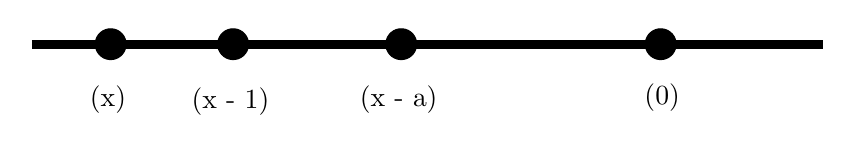
\begin{tikzpicture}[x=0.75pt,y=0.75pt,yscale=-1,xscale=1]
%uncomment if require: \path (0,300); %set diagram left start at 0, and has height of 300


%Straight Lines [id:da22332223838056997] 
\draw [color={rgb, 255:red, 0; green, 0; blue, 0 }  ,draw opacity=1 ][fill={rgb, 255:red, 0; green, 0; blue, 0 }  ,fill opacity=1 ][line width=3]    (99.3,100.47) -- (480.3,100.47) ;


%Shape: Circle [id:dp6643237363432828] 
\draw  [fill={rgb, 255:red, 0; green, 0; blue, 0 }  ,fill opacity=1 ] (129.89,99.88) .. controls (130.16,95.8) and (133.69,92.7) .. (137.78,92.98) .. controls (141.87,93.25) and (144.96,96.78) .. (144.69,100.87) .. controls (144.42,104.96) and (140.88,108.05) .. (136.79,107.78) .. controls (132.71,107.5) and (129.61,103.97) .. (129.89,99.88) -- cycle ;
%Shape: Circle [id:dp3426760131435296] 
\draw  [fill={rgb, 255:red, 0; green, 0; blue, 0 }  ,fill opacity=1 ] (188.89,99.88) .. controls (189.16,95.8) and (192.69,92.7) .. (196.78,92.98) .. controls (200.87,93.25) and (203.96,96.78) .. (203.69,100.87) .. controls (203.42,104.96) and (199.88,108.05) .. (195.79,107.78) .. controls (191.71,107.5) and (188.61,103.97) .. (188.89,99.88) -- cycle ;
%Shape: Circle [id:dp29970333704367036] 
\draw  [fill={rgb, 255:red, 0; green, 0; blue, 0 }  ,fill opacity=1 ] (269.89,99.88) .. controls (270.16,95.8) and (273.69,92.7) .. (277.78,92.98) .. controls (281.87,93.25) and (284.96,96.78) .. (284.69,100.87) .. controls (284.42,104.96) and (280.88,108.05) .. (276.79,107.78) .. controls (272.71,107.5) and (269.61,103.97) .. (269.89,99.88) -- cycle ;
%Shape: Circle [id:dp5094461474575767] 
\draw  [fill={rgb, 255:red, 0; green, 0; blue, 0 }  ,fill opacity=1 ] (394.89,99.88) .. controls (395.16,95.8) and (398.69,92.7) .. (402.78,92.98) .. controls (406.87,93.25) and (409.96,96.78) .. (409.69,100.87) .. controls (409.42,104.96) and (405.88,108.05) .. (401.79,107.78) .. controls (397.71,107.5) and (394.61,103.97) .. (394.89,99.88) -- cycle ;

% Text Node
\draw (136,127) node  [align=left] {(x)};
% Text Node
\draw (195,128) node  [align=left] {(x - 1)};
% Text Node
\draw (276,127) node  [align=left] {(x - a)};
% Text Node
\draw (403,126) node  [align=left] {(0)};


\end{tikzpicture}

    \caption{Visualization of \(\mathbb{A}_{\mathbb{C}}^1\).}
    \label{fig:Affine line}
\end{figure}
\end{center}
\end{example}



%\include{AppendixB}
\backmatter
\begin{thebibliography}{}

\bibitem[Caz]{Cazanave} 
Cristophe Cazanave. 
\textit{Algebraic homotopyclasses of rational functions}. \\
Ann. Scient. Éc. Norm. Sup. 4e série, t. 45, 2012, p. 511 à 534 \\

\bibitem[E-H]{Eisenbud-Harris}
David Eisenbud and Joe Harris.
\textit{The geometry of schemes} \\
Graduate textd in mathematics: 197, Springer verlag, 2000 \\

\bibitem[Har]{hartshorne}
Robin Hartshorne.
\textit{Algebraic geometry} \\
Graduate texts in mathematics: 52, Springer verlag 1977 \\

\bibitem[Hsu]{hsu}
Tim Hsu.
\textit{Applied industrial algebra} \\
http://timhsu.net/courses/127/applied-industrial-algebra.pdf \\

\bibitem[Jan]{Janson}
Svante Janson.
\textit{Resultant and discriminant of polynomials}.\\
http://www2.math.uu.se/~svante/papers/sjN5.pdf \\

\bibitem[Mum]{Mumford1}
David Mumford.
\textit{The red book of varieties and schemes: Second, Expanded Edition}. \\
Lecture notes in mathematics: 1358, Springer verlag, 1999 \\

\bibitem[Vak]{Vakil}
Ravi Vakil.
\textit{The rising sea: Foundations of Algebraic Geometry}.\\
math216.wordpress.com, December 30, 2014 draft \\

%\bibitem[Mum]{Mumford2}
%David Mumford.
%\textit{Introduction to algebraic geometry}.\\
%add publication

\bibitem[W-G]{Wedhorn-Gortz}
Torsten Wedhorn and Ulrich Görtz.
\textit{Algebraic Geometry 1: Schemes} \\
Vieweg+Taubner verlag, 2010

\end{thebibliography} %wohoo works now!

\end{document}
